\documentclass[11pt,preprint, authoryear]{elsarticle}

\usepackage{lmodern}
%%%% My spacing
\usepackage{setspace}
\setstretch{1.2}
\DeclareMathSizes{12}{14}{10}{10}

% Wrap around which gives all figures included the [H] command, or places it "here". This can be tedious to code in Rmarkdown.
\usepackage{float}
\let\origfigure\figure
\let\endorigfigure\endfigure
\renewenvironment{figure}[1][2] {
    \expandafter\origfigure\expandafter[H]
} {
    \endorigfigure
}

\let\origtable\table
\let\endorigtable\endtable
\renewenvironment{table}[1][2] {
    \expandafter\origtable\expandafter[H]
} {
    \endorigtable
}


\usepackage{ifxetex,ifluatex}
\usepackage{fixltx2e} % provides \textsubscript
\ifnum 0\ifxetex 1\fi\ifluatex 1\fi=0 % if pdftex
  \usepackage[T1]{fontenc}
  \usepackage[utf8]{inputenc}
\else % if luatex or xelatex
  \ifxetex
    \usepackage{mathspec}
    \usepackage{xltxtra,xunicode}
  \else
    \usepackage{fontspec}
  \fi
  \defaultfontfeatures{Mapping=tex-text,Scale=MatchLowercase}
  \newcommand{\euro}{€}
\fi

\usepackage{amssymb, amsmath, amsthm, amsfonts}

\def\bibsection{\section*{References}} %%% Make "References" appear before bibliography


\usepackage[round]{natbib}

\usepackage{longtable}
\usepackage[margin=2.3cm,bottom=2cm,top=2.5cm, includefoot]{geometry}
\usepackage{fancyhdr}
\usepackage[bottom, hang, flushmargin]{footmisc}
\usepackage{graphicx}
\numberwithin{equation}{section}
\numberwithin{figure}{section}
\numberwithin{table}{section}
\setlength{\parindent}{0cm}
\setlength{\parskip}{1.3ex plus 0.5ex minus 0.3ex}
\usepackage{textcomp}
\renewcommand{\headrulewidth}{0.2pt}
\renewcommand{\footrulewidth}{0.3pt}

\usepackage{array}
\newcolumntype{x}[1]{>{\centering\arraybackslash\hspace{0pt}}p{#1}}

%%%%  Remove the "preprint submitted to" part. Don't worry about this either, it just looks better without it:
\makeatletter
\def\ps@pprintTitle{%
  \let\@oddhead\@empty
  \let\@evenhead\@empty
  \let\@oddfoot\@empty
  \let\@evenfoot\@oddfoot
}
\makeatother

 \def\tightlist{} % This allows for subbullets!

\usepackage{hyperref}
\hypersetup{breaklinks=true,
            bookmarks=true,
            colorlinks=true,
            citecolor=blue,
            urlcolor=blue,
            linkcolor=blue,
            pdfborder={0 0 0}}


% The following packages allow huxtable to work:
\usepackage{siunitx}
\usepackage{multirow}
\usepackage{hhline}
\usepackage{calc}
\usepackage{tabularx}
\usepackage{booktabs}
\usepackage{caption}


\newenvironment{columns}[1][]{}{}

\newenvironment{column}[1]{\begin{minipage}{#1}\ignorespaces}{%
\end{minipage}
\ifhmode\unskip\fi
\aftergroup\useignorespacesandallpars}

\def\useignorespacesandallpars#1\ignorespaces\fi{%
#1\fi\ignorespacesandallpars}

\makeatletter
\def\ignorespacesandallpars{%
  \@ifnextchar\par
    {\expandafter\ignorespacesandallpars\@gobble}%
    {}%
}
\makeatother

\newlength{\cslhangindent}
\setlength{\cslhangindent}{1.5em}
\newenvironment{CSLReferences}%
  {\setlength{\parindent}{0pt}%
  \everypar{\setlength{\hangindent}{\cslhangindent}}\ignorespaces}%
  {\par}


\urlstyle{same}  % don't use monospace font for urls
\setlength{\parindent}{0pt}
\setlength{\parskip}{6pt plus 2pt minus 1pt}
\setlength{\emergencystretch}{3em}  % prevent overfull lines
\setcounter{secnumdepth}{5}

%%% Use protect on footnotes to avoid problems with footnotes in titles
\let\rmarkdownfootnote\footnote%
\def\footnote{\protect\rmarkdownfootnote}
\IfFileExists{upquote.sty}{\usepackage{upquote}}{}

%%% Include extra packages specified by user

%%% Hard setting column skips for reports - this ensures greater consistency and control over the length settings in the document.
%% page layout
%% paragraphs
\setlength{\baselineskip}{12pt plus 0pt minus 0pt}
\setlength{\parskip}{12pt plus 0pt minus 0pt}
\setlength{\parindent}{0pt plus 0pt minus 0pt}
%% floats
\setlength{\floatsep}{12pt plus 0 pt minus 0pt}
\setlength{\textfloatsep}{20pt plus 0pt minus 0pt}
\setlength{\intextsep}{14pt plus 0pt minus 0pt}
\setlength{\dbltextfloatsep}{20pt plus 0pt minus 0pt}
\setlength{\dblfloatsep}{14pt plus 0pt minus 0pt}
%% maths
\setlength{\abovedisplayskip}{12pt plus 0pt minus 0pt}
\setlength{\belowdisplayskip}{12pt plus 0pt minus 0pt}
%% lists
\setlength{\topsep}{10pt plus 0pt minus 0pt}
\setlength{\partopsep}{3pt plus 0pt minus 0pt}
\setlength{\itemsep}{5pt plus 0pt minus 0pt}
\setlength{\labelsep}{8mm plus 0mm minus 0mm}
\setlength{\parsep}{\the\parskip}
\setlength{\listparindent}{\the\parindent}
%% verbatim
\setlength{\fboxsep}{5pt plus 0pt minus 0pt}



\begin{document}



%titlepage
\thispagestyle{empty}
\begin{center}
\begin{minipage}{0.75\linewidth}
    \centering
%Entry1
    {\uppercase{\huge Real Exchange Rate Behaviour: A Replication and
Robustness Check\par}}
    \vspace{2cm}
%Author's name
    {\LARGE Cassandra Pengelly \textbar{} 20346212\par}
    \vspace{1cm}
%University logo
\begin{center}
    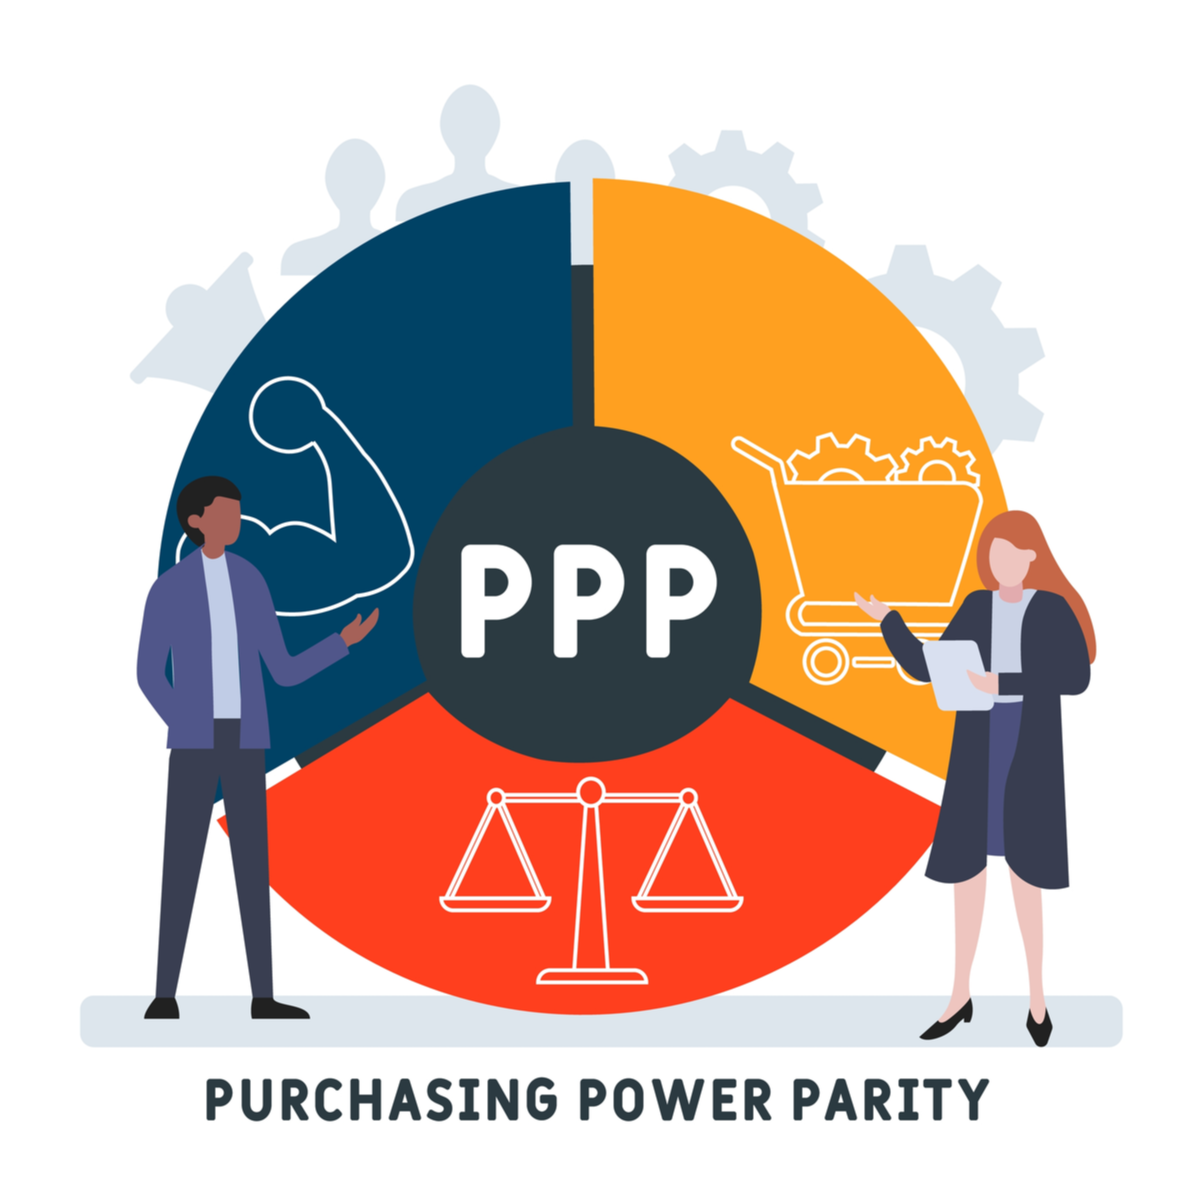
\includegraphics[width=0.5\linewidth]{Tex/Logo.png}
\end{center}
\vspace{1cm}
%Supervisor's Details
\begin{center}
    {\Large Econometrics 871: Time Series Project\par}
    \vspace{1cm}
%Degree
    {\large \par}
    \vspace{1cm}
%Institution
    {\large \par}
    \vspace{1cm}
%Date
    {\large }
%More
    {\normalsize }
%More
    {\normalsize }
\end{center}
\end{minipage}
\end{center}
\clearpage


\begin{frontmatter}  %

\title{}

% Set to FALSE if wanting to remove title (for submission)


\vspace{1cm}





\vspace{0.5cm}

\end{frontmatter}


\renewcommand{\contentsname}{Table of Contents}
{\tableofcontents}

%________________________
% Header and Footers
%%%%%%%%%%%%%%%%%%%%%%%%%%%%%%%%%
\pagestyle{fancy}
\chead{}
\rhead{}
\lfoot{}
\rfoot{\footnotesize Page \thepage}
\lhead{}
%\rfoot{\footnotesize Page \thepage } % "e.g. Page 2"
\cfoot{}

%\setlength\headheight{30pt}
%%%%%%%%%%%%%%%%%%%%%%%%%%%%%%%%%
%________________________

\headsep 35pt % So that header does not go over title




\newpage

\hypertarget{introduction}{%
\section{\texorpdfstring{Introduction
\label{Introduction}}{Introduction }}\label{introduction}}

How do we compare living standards and economic productivity between
countries? This is one of the questions that macroeconomics attempts to
answers and a number of tools have been developed within the field to
this end. One of these tools is the Purchasing Power Parity (PPP)
theory, which uses a basket of goods to compare the currencies of
different countries. This theory has been widely tested using data, and
the results have been divisive and somewhat puzzling
(\protect\hyperlink{ref-puz}{El-Gamal \& Ryu}
(\protect\hyperlink{ref-puz}{2006})).

In this essay, I replicate\footnote{More accurately, try my best to
  replicate} the paper ``Real Exchange Rate Behaviour: Evidence from
Black Markets'' by \protect\hyperlink{ref-Kul}{Luintel}
(\protect\hyperlink{ref-Kul}{2000}), which tests the PPP hypothesis.
\protect\hyperlink{ref-Kul}{Luintel} (\protect\hyperlink{ref-Kul}{2000})
finds that the behaviour of the real exchange rate is mean-reverting in
the long-run, which suggests that the PPP theory is empirically
supported. I include some other tests in addition to those presented in
the paper as a robustness check on these results.

This essay\footnote{This essay was written in R using the package by
  \protect\hyperlink{ref-Texevier}{Katzke}
  (\protect\hyperlink{ref-Texevier}{2017})} is organised as follows.
Section \ref{Context} contextualises Luintel's paper and discusses the
robustness checks. Section \ref{Data} discusses the data and reports the
results of the Wald-Wolfowitz tests. Section \ref{Unit} deals with the
unit root tests. Section \ref{Var} reports the results of the variance
ratio test.The code for this replication can be found on Github
\href{https://github.com/cass-code/metrics.git}{here}.

\hypertarget{context-and-evaluation}{%
\section{\texorpdfstring{Context and Evaluation
\label{Context}}{Context and Evaluation }}\label{context-and-evaluation}}

\protect\hyperlink{ref-Kul}{Luintel} (\protect\hyperlink{ref-Kul}{2000})
investigates whether the PPP hypothesis holds empirically. To test this
theory, \protect\hyperlink{ref-Kul}{Luintel}
(\protect\hyperlink{ref-Kul}{2000}) uses monthly black market real
exchange rates (in terms of the US dollar) from eight developing Asian
countries: India, Sri Lanka, Myanmar, Malaysia, Pakistan, Philippines,
Taiwan and Thailand. Using data from developing countries (rather than
from developed countries) was a novel approach for its time. The black
market rates are used as a proxy for the float rates of developing
countries.

Practically, the paper has two main aims: the first is to determine
whether there are segmented trends in the data, and the second is to
test whether the panel data is stationary. At the time that this paper
was written (early 2000s), the puzzle of PPP was that tests for unit
roots failed to reject the null hypothesis. The null hypothesis in these
cases was the presence of unit roots; these tests implied
non-stationarity and discredited PPP, despite the support from economic
theory(\protect\hyperlink{ref-puz}{El-Gamal \& Ryu}
(\protect\hyperlink{ref-puz}{2006})).

\protect\hyperlink{ref-Kul}{Luintel} (\protect\hyperlink{ref-Kul}{2000})
makes use of (more) powerful unit root tests for heterogeneous panels,
and finds that real exchange rates are mean-reverting. This was novel
for the time as most time-series studies rejected PPP and concluded that
the real exchange rate followed a random walk. This suggested that any
shocks to the real exchange rate were persistent and there was no
mean-reversion either in the short or long term
(\protect\hyperlink{ref-rog}{Rogoff}
(\protect\hyperlink{ref-rog}{1996})).
\protect\hyperlink{ref-Kul}{Luintel} (\protect\hyperlink{ref-Kul}{2000})
finds that the black market real exchange rates do not behave in an
excessively volatile manner, which conflicted with the findings of the
literature at that time. Additionally, the findings of the study implied
that such empirical investigation may not necessarily suffer from
survivorship bias.

A critical part of Luintel's paper is testing for unit roots in the
panel data, specifically the paper makes use of the Im-Pesaran-Shin
T-bar test. In addition to replicating this test, I implement several
other unit root tests as a robustness check and find that the results
are mixed. \protect\hyperlink{ref-Kul}{Luintel}
(\protect\hyperlink{ref-Kul}{2000: 70}) defends the choice of the IPS
tests well, citing that they allow for the dynamics and error variances
across groups, and the T-bar tests based on meaned regressions are
valid. Additionally, these tests may have better small sample
propoerties. I run the IPS tests using
\protect\hyperlink{ref-Kul}{Luintel}
(\protect\hyperlink{ref-Kul}{2000})'s specified lags, and the AIC
method. I then implement the panel stationarity tests proposed by
\protect\hyperlink{ref-lev}{Levin, Lin \& James Chu}
(\protect\hyperlink{ref-lev}{2002}), \protect\hyperlink{ref-wu}{Maddala
\& Wu} (\protect\hyperlink{ref-wu}{1999}),
\protect\hyperlink{ref-had}{Hadri} (\protect\hyperlink{ref-had}{2002}),
as well as a bootstrapped panel unit root test from
\protect\hyperlink{ref-pal}{Palm, Smeekes \& Urbain}
(\protect\hyperlink{ref-pal}{2011}).

\hypertarget{data}{%
\section{\texorpdfstring{Data \label{Data}}{Data }}\label{data}}

The data used for the analysis is a series on black market nominal
exchange rates and consumer price indices (CPI) for 8 developing Asian
countries, namely: India, Sri Lanka, Myanmar, Malaysia, Pakistan,
Philippines, Taiwan and Thailand. I take a subset of these countries by
excluding Taiwan\footnote{I excluded Taiwan because there is some data
  missing from the set and I don't know how to adjust an unbalanced
  panel. However, it is also interesting to test if the results hold
  when taking a subset} from the analysis.
\protect\hyperlink{ref-Kul}{Luintel} (\protect\hyperlink{ref-Kul}{2000})
sources data from various issues of \emph{Pick's Currency Year Book} and
\emph{World Currency Year Book}. The data used for Luintel's paper is
accessible through the Journal of Applied Econometrics archive, which is
where I attained my data. The sample period runs for 31 periods from
January 1958 to June 1989. This sample period is split into two parts:
Bretton Woods and after Bretton Woods (also referred to as pre-float
period and the float period).

The nominal exchange rates are units currencies per unit of US dollar.
There were two mistakes in the nominal exchange rate datasets: for
Myanmar November 1974, there was a value of 1.45, which I replaced with
16.5 (based on interpolation). And for the Philippines in September
1975, there was a value of 0.7 with which I replaced with 7.7 (based on
interpolation).\footnote{I discovered these mistakes when there was a
  dramatic difference in my plots of the real exchange rates and
  Luintel's plots.} Luintel sources the CPI figures from issues of
International Financial Statistics (which are included in Luintel's
dataset available in the JAE data archives).

To calculate the real exchange rates, I follow the lead of
\protect\hyperlink{ref-Kul}{Luintel} (\protect\hyperlink{ref-Kul}{2000:
165}) and apply the following formula to the nominal exchange rates:

\[
rex = log(Nominal Exchange Rate) - log(CPI) + log(United States CPI)
\]

I plot the real exchange rate series below in \ref{Figure1}. The plots
below match those of \protect\hyperlink{ref-Kul}{Luintel}
(\protect\hyperlink{ref-Kul}{2000: 166}) and indicate that the real
exchange rates are trending. Additionally, the graphs show that the
black market exchange rates are somewhat volatile. As expected, we see
that after the first oil shock of 1973 the currencies appreciated and
then slowly reverted. The plots suggest that the trends are segmented.
\protect\hyperlink{ref-Kul}{Luintel} (\protect\hyperlink{ref-Kul}{2000:
169}) tests this hypothesis using formal tests, and I follow suit - the
results of the Wald-Wolfowitz Tests are reported below the plots in
\ref{wald}.

\begin{center}\includegraphics{20346212_files/figure-latex/Figure1-1} \end{center}

\begin{figure}[H]

{\centering \includegraphics{20346212_files/figure-latex/Figure2-1} 

}

\caption{Plot of Real Exchange Rates over Time\label{Figure1}}\label{fig:Figure2}
\end{figure}

\hypertarget{wald-wolfowitz-tests}{%
\subsection{\texorpdfstring{Wald-Wolfowitz Tests
\label{wald}}{Wald-Wolfowitz Tests }}\label{wald-wolfowitz-tests}}

\begin{table}[H]
\centering
\caption{Wald-Wolfowitz tests \label{tab1}} 
\begin{tabular}{lrrrrrrr}
  \hline
Test/Country & India & SriLanka & Malaysia & Myanmar & Pakistan & Philippines & Thailand \\ 
  \hline
Wald-Wolfowitz & -16.07 & -18.54 & -17.10 & -18.23 & -16.27 & -17.10 & -15.96 \\ 
   \hline
\end{tabular}
\end{table}

\hypertarget{unit-root-tests}{%
\section{\texorpdfstring{Unit Root Tests
\label{Unit}}{Unit Root Tests }}\label{unit-root-tests}}

First, I employed the Augmented Dickey-Fuller test for the individual
exchange rates to see whether there was a unit root present. The test
results show that the individual time series are all non-stationary.

\begingroup\fontsize{11pt}{12pt}\selectfont
\begin{longtable}{lrrr}
\caption{Augmented Dickey-Fuller Tests} \\ 
  \toprule
Countries & Full Sample & Bretton Woods (1958:1-1973:3) & Post-Bretton Woods (1973:4-1989:6) \\ 
  \hline 
\endhead 
\hline 
{\footnotesize Continued on next page} 
\endfoot 
\endlastfoot 
 \midrule
India (Rupee) & -2.70 & -2.07 & -3.66 \\ 
  Sri Lanka (Rupee) & -3.22 & -2.11 & -2.44 \\ 
  Malaysia (Ringgit) & -1.47 & -2.16 & -3.77 \\ 
  Myanmar (Kyat) & -1.53 & -1.71 & -0.16 \\ 
  Pakistan (Rupee) & -3.35 & -2.97 & -5.91 \\ 
  Phillipines (Peso) & -3.09 & -2.07 & -3.38 \\ 
  Thailand (Baht) & -2.44 & -3.36 & -3.93 \\ 
   \bottomrule
\end{longtable}
\endgroup

\hypertarget{panel-unit-root-tests}{%
\subsection{Panel Unit Root Tests}\label{panel-unit-root-tests}}

As noted by \protect\hyperlink{ref-pes}{Breitung \& Pesaran}
(\protect\hyperlink{ref-pes}{2005: 18}), when using country data for
macroeconomic applications, there are often contemporaneous correlations
within the time series, which is a relevant concern for testing the PPP
hypothesis. There may be unobserved common factors or spatial spillover
effects, which need to be accounted for in the unit root test. Modelling
cross section dependence in panel data sets is still an emerging field,
but \protect\hyperlink{ref-im}{Pasaran, Im \& Shin}
(\protect\hyperlink{ref-im}{1997}) suggest that the appropriate test
statistic is the T-bar test based on cross-sectional demeaned
regressions. This is the approach that I take below (Im-Pesaran-Shin
T-bar test), and the test rejects the null hypothesis at a 1\% level,
both when including and excluding a trend. This supports the results of
\protect\hyperlink{ref-Kul}{Luintel} (\protect\hyperlink{ref-Kul}{2000:
173}). I use the same lags as \protect\hyperlink{ref-Kul}{Luintel}
(\protect\hyperlink{ref-Kul}{2000}) for the first IPS T-bar test, are
for the full sample: Malaysia(l) and Thailand(1), for the Bretton Woods
period: Thailand(1), and for the post Bretton Woods period: Malaysia(l)
and Thailand(1).

The first unit root test I employ is the Im-Pesaran-Shin t-bar test to
replicate \protect\hyperlink{ref-Kul}{Luintel}
(\protect\hyperlink{ref-Kul}{2000}) test. The results below show that
the null hypothesis (there exists a unit root) is rejected at the
conventional levels of significance\footnote{I found out this is a fancy
  way of saying reject at 1\% and 5\%} \ref{ips}

\begingroup\fontsize{12pt}{13pt}\selectfont
\begin{longtable}{llrll}
\caption{IPS Panel Unit Root Tests (Tbar)} \\ 
  \toprule
Period & Test & T-statistic & Trend & Outcome \\ 
  \hline 
\endhead 
\hline 
{\footnotesize Continued on next page} 
\endfoot 
\endlastfoot 
 \midrule
Full Sample & IPS & -2.97 & Yes & Reject H0 \\ 
   & IPS & -2.56 & No & Reject H0 \\ 
  Bretton Woods & IPS & -2.47 & Yes & Reject H0 \\ 
   & IPS & -1.74 & No & Reject H0 \\ 
  Post Bretton Woods & IPS & -2.53 & Yes & Reject H0 \\ 
   & IPS & -2.65 & No & Reject H0 \\ 
   \bottomrule
\label{ips}
\end{longtable}
\endgroup

I then tests for unit roots using LLL test (I used the package by
\protect\hyperlink{ref-plm}{Millo} (\protect\hyperlink{ref-plm}{2017})
for this).

The function panel\_test performs a test on a multivariate (panel) time
series by testing the null hypothesis that all series have a unit root.
A rejection is typically interpreted as evidence that a `significant
proportion' of the series is stationary, although how large that
proportion is - or which series are stationary - is not given by the
test. The test is based on averaging the individual test statistics,
also called the Group-Mean (GM) test in Palm, Smeekes and Urbain (2011).

\hypertarget{variance-ratio-test}{%
\section{\texorpdfstring{Variance Ratio Test
\label{Var}}{Variance Ratio Test }}\label{variance-ratio-test}}

The following table shows results of the Variance Ratio test for the
full sample for up to 20 months. The results of the variance ratio test
for the Bretton Woods period and post Bretton Woods period (for up to 20
months\footnote{The results for 190 months is available upon request; it
  has been omitted purely to save space}) can be found in the Appendix
(\ref{A})

\begingroup\fontsize{12pt}{13pt}\selectfont
\begin{longtable}{lrrrrrrr}
\caption{Variance Ratio Test for Full Sample Up to month 20} \\ 
  \toprule
Months & India & SriLanka & Malaysia & Myanmar & Pakistan & Philippines & Thailand \\ 
  \hline 
\endhead 
\hline 
{\footnotesize Continued on next page} 
\endfoot 
\endlastfoot 
 \midrule
1 & 1.00 & 1.00 & 1.00 & 1.00 & 1.00 & 1.00 & 1.00 \\ 
  se & 0.10 & 0.10 & 0.10 & 0.10 & 0.10 & 0.10 & 0.10 \\ 
  2 & 1.00 & 0.95 & 0.79 & 1.04 & 0.91 & 0.91 & 0.74 \\ 
  se & 0.10 & 0.10 & 0.10 & 0.10 & 0.10 & 0.10 & 0.10 \\ 
  3 & 1.02 & 0.86 & 0.79 & 1.05 & 0.81 & 0.86 & 0.68 \\ 
  se & 0.10 & 0.10 & 0.10 & 0.10 & 0.10 & 0.10 & 0.10 \\ 
  4 & 1.01 & 0.87 & 0.75 & 1.00 & 0.71 & 0.82 & 0.58 \\ 
  se & 0.10 & 0.10 & 0.10 & 0.10 & 0.10 & 0.10 & 0.10 \\ 
  5 & 0.95 & 0.89 & 0.73 & 0.98 & 0.65 & 0.80 & 0.52 \\ 
  se & 0.10 & 0.10 & 0.10 & 0.10 & 0.10 & 0.10 & 0.10 \\ 
  6 & 0.91 & 0.90 & 0.73 & 0.95 & 0.61 & 0.77 & 0.48 \\ 
  se & 0.10 & 0.10 & 0.10 & 0.10 & 0.10 & 0.10 & 0.10 \\ 
  7 & 0.86 & 0.91 & 0.69 & 0.93 & 0.58 & 0.76 & 0.44 \\ 
  se & 0.10 & 0.10 & 0.10 & 0.10 & 0.10 & 0.10 & 0.10 \\ 
  8 & 0.83 & 0.90 & 0.69 & 0.92 & 0.56 & 0.77 & 0.42 \\ 
  se & 0.10 & 0.10 & 0.10 & 0.10 & 0.10 & 0.10 & 0.10 \\ 
  9 & 0.81 & 0.89 & 0.66 & 0.90 & 0.53 & 0.81 & 0.40 \\ 
  se & 0.10 & 0.10 & 0.10 & 0.10 & 0.10 & 0.10 & 0.10 \\ 
  10 & 0.81 & 0.88 & 0.63 & 0.89 & 0.50 & 0.79 & 0.39 \\ 
  se & 0.10 & 0.10 & 0.10 & 0.10 & 0.10 & 0.10 & 0.10 \\ 
  11 & 0.81 & 0.88 & 0.61 & 0.91 & 0.49 & 0.79 & 0.37 \\ 
  se & 0.10 & 0.10 & 0.10 & 0.10 & 0.10 & 0.10 & 0.10 \\ 
  12 & 0.83 & 0.88 & 0.57 & 0.95 & 0.46 & 0.78 & 0.37 \\ 
  se & 0.10 & 0.10 & 0.10 & 0.10 & 0.10 & 0.10 & 0.10 \\ 
  13 & 0.86 & 0.87 & 0.57 & 0.96 & 0.47 & 0.79 & 0.37 \\ 
  se & 0.10 & 0.10 & 0.10 & 0.10 & 0.10 & 0.10 & 0.10 \\ 
  14 & 0.88 & 0.87 & 0.57 & 0.98 & 0.48 & 0.79 & 0.37 \\ 
  se & 0.10 & 0.10 & 0.10 & 0.10 & 0.10 & 0.10 & 0.10 \\ 
  15 & 0.90 & 0.88 & 0.57 & 1.00 & 0.48 & 0.80 & 0.37 \\ 
  se & 0.10 & 0.10 & 0.10 & 0.10 & 0.10 & 0.10 & 0.10 \\ 
  16 & 0.92 & 0.88 & 0.57 & 1.02 & 0.49 & 0.79 & 0.37 \\ 
  se & 0.10 & 0.10 & 0.10 & 0.10 & 0.10 & 0.10 & 0.10 \\ 
  17 & 0.92 & 0.89 & 0.58 & 1.03 & 0.49 & 0.78 & 0.36 \\ 
  se & 0.10 & 0.10 & 0.10 & 0.10 & 0.10 & 0.10 & 0.10 \\ 
  18 & 0.92 & 0.88 & 0.59 & 1.04 & 0.49 & 0.77 & 0.36 \\ 
  se & 0.10 & 0.10 & 0.10 & 0.10 & 0.10 & 0.10 & 0.10 \\ 
  19 & 0.91 & 0.88 & 0.60 & 1.05 & 0.50 & 0.76 & 0.36 \\ 
  se & 0.10 & 0.10 & 0.10 & 0.10 & 0.10 & 0.10 & 0.10 \\ 
  20 & 0.90 & 0.87 & 0.62 & 1.08 & 0.52 & 0.75 & 0.36 \\ 
  se & 0.10 & 0.10 & 0.10 & 0.10 & 0.10 & 0.10 & 0.10 \\ 
   \bottomrule
\end{longtable}
\endgroup

\hypertarget{conclusion}{%
\section{Conclusion}\label{conclusion}}

\newpage

\hypertarget{references}{%
\section*{References}\label{references}}
\addcontentsline{toc}{section}{References}

\hypertarget{refs}{}
\begin{CSLReferences}{1}{0}
\leavevmode\hypertarget{ref-pes}{}%
Breitung, J. \& Pesaran, M.H. 2005. \emph{Unit roots and cointegration
in panels}. Deutsche Bundesbank. {[}Online{]}, Available:
\url{https://ideas.repec.org/p/zbw/bubdp1/4236.html}.

\leavevmode\hypertarget{ref-puz}{}%
El-Gamal, M.A. \& Ryu, D. 2006. Short-memory and the PPP hypothesis.
\emph{Journal of Economic Dynamics and Control}. 30(3):361--391.
{[}Online{]}, Available:
\url{http://www.sciencedirect.com/science/article/B6V85-4HD8B3Y-1/1/b7865989592c6f1ee4b79a80036183c9}.

\leavevmode\hypertarget{ref-had}{}%
Hadri, K. 2002. Testing for stationarity in heterogeneous panel data.
\emph{The Econometrics Journal}. 3(2):148--161.

\leavevmode\hypertarget{ref-Texevier}{}%
Katzke, N.F. 2017. \emph{{Texevier}: {P}ackage to create elsevier
templates for rmarkdown}. Stellenbosch, South Africa: Bureau for
Economic Research.

\leavevmode\hypertarget{ref-lev}{}%
Levin, A., Lin, C.-F. \& James Chu, C.-S. 2002. Unit root tests in panel
data: Asymptotic and finite-sample properties. \emph{Journal of
Econometrics}. 108(1):1--24. {[}Online{]}, Available:
\url{https://EconPapers.repec.org/RePEc:eee:econom:v:108:y:2002:i:1:p:1-24}.

\leavevmode\hypertarget{ref-Kul}{}%
Luintel, K.B. 2000. Real exchange rate behaviour: Evidence from black
markets. \emph{Journal of Applied Econometrics}. 15(2):161--185.
{[}Online{]}, Available: \url{http://www.jstor.org/stable/2678529}.

\leavevmode\hypertarget{ref-wu}{}%
Maddala, G.S. \& Wu, S. 1999. A comparative study of unit root tests
with panel data and a new simple test. \emph{Oxford Bulletin of
Economics and Statistics}. 61(S1):631--652. {[}Online{]}, Available:
\url{https://EconPapers.repec.org/RePEc:bla:obuest:v:61:y:1999:i:s1:p:631-652}.

\leavevmode\hypertarget{ref-plm}{}%
Millo, G. 2017. Robust standard error estimators for panel models: A
unifying approach. \emph{Journal of Statistical Software}. 82(3):1--27.

\leavevmode\hypertarget{ref-pal}{}%
Palm, F., Smeekes, S. \& Urbain, J.-P. 2011. Cross-sectional dependence
robust block bootstrap panel unit root tests. \emph{Journal of
Econometrics}. 163(1):85--104. {[}Online{]}, Available:
\url{https://EconPapers.repec.org/RePEc:eee:econom:v:163:y:2011:i:1:p:85-104}.

\leavevmode\hypertarget{ref-im}{}%
Pasaran, M.H., Im, K.S. \& Shin, Y. 1997. \emph{Testing for unit roots
in heterogeneous panels}. Faculty of Economics, University of Cambridge.
{[}Online{]}, Available:
\url{https://EconPapers.repec.org/RePEc:cam:camdae:9526}.

\leavevmode\hypertarget{ref-rog}{}%
Rogoff, K. 1996. The purchasing power parity puzzle. \emph{Journal of
Economic Literature}. 34:647--68.

\end{CSLReferences}

\newpage

\hypertarget{appendix}{%
\section*{\texorpdfstring{Appendix:
\label{A}}{Appendix: }}\label{appendix}}
\addcontentsline{toc}{section}{Appendix: \label{A}}

\begingroup\fontsize{12pt}{13pt}\selectfont
\begin{longtable}{lrrrrrrr}
\caption{Variance Ratio Test for Bretton Woods period up to month 20} \\ 
  \toprule
Months & India & SriLanka & Malaysia & Myanmar & Pakistan & Philippines & Thailand \\ 
  \hline 
\endhead 
\hline 
{\footnotesize Continued on next page} 
\endfoot 
\endlastfoot 
 \midrule
1 & 1.00 & 1.00 & 1.00 & 1.00 & 1.00 & 1.00 & 1.00 \\ 
  se & 0.15 & 0.15 & 0.15 & 0.15 & 0.15 & 0.15 & 0.15 \\ 
  2 & 1.06 & 0.88 & 0.80 & 1.03 & 1.01 & 1.02 & 0.79 \\ 
  se & 0.15 & 0.15 & 0.15 & 0.15 & 0.15 & 0.15 & 0.15 \\ 
  3 & 1.03 & 0.80 & 0.73 & 1.01 & 0.92 & 0.90 & 0.72 \\ 
  se & 0.15 & 0.15 & 0.15 & 0.15 & 0.15 & 0.15 & 0.15 \\ 
  4 & 0.99 & 0.77 & 0.66 & 0.95 & 0.76 & 0.84 & 0.61 \\ 
  se & 0.15 & 0.15 & 0.15 & 0.15 & 0.15 & 0.15 & 0.15 \\ 
  5 & 0.92 & 0.79 & 0.59 & 0.93 & 0.61 & 0.81 & 0.50 \\ 
  se & 0.15 & 0.15 & 0.15 & 0.15 & 0.15 & 0.15 & 0.15 \\ 
  6 & 0.88 & 0.80 & 0.56 & 0.91 & 0.55 & 0.79 & 0.47 \\ 
  se & 0.15 & 0.15 & 0.15 & 0.15 & 0.15 & 0.15 & 0.15 \\ 
  7 & 0.84 & 0.80 & 0.53 & 0.90 & 0.50 & 0.79 & 0.39 \\ 
  se & 0.15 & 0.15 & 0.15 & 0.15 & 0.15 & 0.15 & 0.15 \\ 
  8 & 0.82 & 0.80 & 0.55 & 0.89 & 0.49 & 0.81 & 0.36 \\ 
  se & 0.15 & 0.15 & 0.15 & 0.15 & 0.15 & 0.15 & 0.15 \\ 
  9 & 0.80 & 0.80 & 0.55 & 0.88 & 0.44 & 0.83 & 0.36 \\ 
  se & 0.15 & 0.15 & 0.15 & 0.15 & 0.15 & 0.15 & 0.15 \\ 
  10 & 0.80 & 0.78 & 0.56 & 0.87 & 0.39 & 0.82 & 0.36 \\ 
  se & 0.15 & 0.15 & 0.15 & 0.15 & 0.15 & 0.15 & 0.15 \\ 
  11 & 0.79 & 0.78 & 0.56 & 0.90 & 0.36 & 0.81 & 0.37 \\ 
  se & 0.15 & 0.15 & 0.15 & 0.15 & 0.15 & 0.15 & 0.15 \\ 
  12 & 0.80 & 0.78 & 0.53 & 0.96 & 0.34 & 0.82 & 0.35 \\ 
  se & 0.15 & 0.15 & 0.15 & 0.15 & 0.15 & 0.15 & 0.15 \\ 
  13 & 0.83 & 0.76 & 0.53 & 0.98 & 0.35 & 0.84 & 0.35 \\ 
  se & 0.15 & 0.15 & 0.15 & 0.15 & 0.15 & 0.15 & 0.15 \\ 
  14 & 0.86 & 0.74 & 0.55 & 1.00 & 0.36 & 0.85 & 0.34 \\ 
  se & 0.15 & 0.15 & 0.15 & 0.15 & 0.15 & 0.15 & 0.15 \\ 
  15 & 0.90 & 0.74 & 0.56 & 1.04 & 0.35 & 0.87 & 0.32 \\ 
  se & 0.15 & 0.15 & 0.15 & 0.15 & 0.15 & 0.15 & 0.15 \\ 
  16 & 0.88 & 0.72 & 0.56 & 1.07 & 0.34 & 0.87 & 0.31 \\ 
  se & 0.15 & 0.15 & 0.15 & 0.15 & 0.15 & 0.15 & 0.15 \\ 
  17 & 0.89 & 0.71 & 0.56 & 1.09 & 0.33 & 0.87 & 0.30 \\ 
  se & 0.15 & 0.15 & 0.15 & 0.15 & 0.15 & 0.15 & 0.15 \\ 
  18 & 0.89 & 0.71 & 0.56 & 1.10 & 0.34 & 0.88 & 0.31 \\ 
  se & 0.15 & 0.15 & 0.15 & 0.15 & 0.15 & 0.15 & 0.15 \\ 
  19 & 0.87 & 0.70 & 0.57 & 1.11 & 0.35 & 0.88 & 0.31 \\ 
  se & 0.15 & 0.15 & 0.15 & 0.15 & 0.15 & 0.15 & 0.15 \\ 
  20 & 0.84 & 0.69 & 0.58 & 1.15 & 0.36 & 0.89 & 0.32 \\ 
  se & 0.15 & 0.15 & 0.15 & 0.15 & 0.15 & 0.15 & 0.15 \\ 
   \bottomrule
\end{longtable}
\endgroup

\begingroup\fontsize{12pt}{13pt}\selectfont
\begin{longtable}{lrrrrrrr}
\caption{Variance Ratio Test for post Bretton Woods period up to 20 months} \\ 
  \toprule
Months & India & SriLanka & Malaysia & Myanmar & Pakistan & Philippines & Thailand \\ 
  \hline 
\endhead 
\hline 
{\footnotesize Continued on next page} 
\endfoot 
\endlastfoot 
 \midrule
1 & 1.00 & 1.00 & 1.00 & 1.00 & 1.00 & 1.00 & 1.00 \\ 
  se & 0.14 & 0.14 & 0.14 & 0.14 & 0.14 & 0.14 & 0.14 \\ 
  2 & 0.95 & 1.01 & 0.78 & 1.05 & 0.78 & 0.85 & 0.71 \\ 
  se & 0.14 & 0.14 & 0.14 & 0.14 & 0.14 & 0.14 & 0.14 \\ 
  3 & 0.99 & 0.91 & 0.80 & 1.14 & 0.68 & 0.84 & 0.66 \\ 
  se & 0.14 & 0.14 & 0.14 & 0.14 & 0.14 & 0.14 & 0.14 \\ 
  4 & 0.98 & 0.93 & 0.75 & 1.14 & 0.61 & 0.82 & 0.58 \\ 
  se & 0.14 & 0.14 & 0.14 & 0.14 & 0.14 & 0.14 & 0.14 \\ 
  5 & 0.93 & 0.94 & 0.76 & 1.12 & 0.60 & 0.81 & 0.53 \\ 
  se & 0.14 & 0.14 & 0.14 & 0.14 & 0.14 & 0.14 & 0.14 \\ 
  6 & 0.88 & 0.94 & 0.73 & 1.06 & 0.54 & 0.78 & 0.49 \\ 
  se & 0.14 & 0.14 & 0.14 & 0.14 & 0.14 & 0.14 & 0.14 \\ 
  7 & 0.82 & 0.94 & 0.69 & 1.02 & 0.50 & 0.76 & 0.45 \\ 
  se & 0.14 & 0.14 & 0.14 & 0.14 & 0.14 & 0.14 & 0.14 \\ 
  8 & 0.77 & 0.92 & 0.68 & 1.00 & 0.45 & 0.76 & 0.44 \\ 
  se & 0.14 & 0.14 & 0.14 & 0.14 & 0.14 & 0.14 & 0.14 \\ 
  9 & 0.75 & 0.89 & 0.62 & 0.98 & 0.40 & 0.81 & 0.40 \\ 
  se & 0.15 & 0.15 & 0.15 & 0.15 & 0.15 & 0.15 & 0.15 \\ 
  10 & 0.75 & 0.86 & 0.60 & 0.98 & 0.39 & 0.79 & 0.38 \\ 
  se & 0.15 & 0.15 & 0.15 & 0.15 & 0.15 & 0.15 & 0.15 \\ 
  11 & 0.75 & 0.85 & 0.55 & 0.98 & 0.38 & 0.79 & 0.34 \\ 
  se & 0.15 & 0.15 & 0.15 & 0.15 & 0.15 & 0.15 & 0.15 \\ 
  12 & 0.76 & 0.84 & 0.51 & 0.99 & 0.37 & 0.78 & 0.33 \\ 
  se & 0.15 & 0.15 & 0.15 & 0.15 & 0.15 & 0.15 & 0.15 \\ 
  13 & 0.76 & 0.82 & 0.47 & 1.00 & 0.39 & 0.78 & 0.32 \\ 
  se & 0.15 & 0.15 & 0.15 & 0.15 & 0.15 & 0.15 & 0.15 \\ 
  14 & 0.75 & 0.83 & 0.45 & 0.99 & 0.40 & 0.77 & 0.32 \\ 
  se & 0.15 & 0.15 & 0.15 & 0.15 & 0.15 & 0.15 & 0.15 \\ 
  15 & 0.73 & 0.83 & 0.43 & 0.98 & 0.39 & 0.77 & 0.31 \\ 
  se & 0.15 & 0.15 & 0.15 & 0.15 & 0.15 & 0.15 & 0.15 \\ 
  16 & 0.72 & 0.83 & 0.42 & 0.99 & 0.39 & 0.75 & 0.31 \\ 
  se & 0.15 & 0.15 & 0.15 & 0.15 & 0.15 & 0.15 & 0.15 \\ 
  17 & 0.72 & 0.83 & 0.42 & 0.98 & 0.38 & 0.74 & 0.30 \\ 
  se & 0.15 & 0.15 & 0.15 & 0.15 & 0.15 & 0.15 & 0.15 \\ 
  18 & 0.71 & 0.81 & 0.42 & 0.98 & 0.38 & 0.72 & 0.28 \\ 
  se & 0.15 & 0.15 & 0.15 & 0.15 & 0.15 & 0.15 & 0.15 \\ 
  19 & 0.68 & 0.80 & 0.42 & 0.99 & 0.38 & 0.70 & 0.27 \\ 
  se & 0.15 & 0.15 & 0.15 & 0.15 & 0.15 & 0.15 & 0.15 \\ 
  20 & 0.64 & 0.78 & 0.41 & 0.99 & 0.39 & 0.68 & 0.25 \\ 
  se & 0.15 & 0.15 & 0.15 & 0.15 & 0.15 & 0.15 & 0.15 \\ 
   \bottomrule
\end{longtable}
\endgroup

\bibliography{Tex/ref}





\end{document}
